\documentclass[10pt, a4paper]{article} % first option = text size, second = paper size, choose "article" for no chapters etc., else choose "report", only use "book" for irl printed book
\usepackage[utf8]{inputenc} % better encoding of input
\usepackage[T1]{fontenc} % better encoding of font
\usepackage{lmodern} % better font
\usepackage[english]{babel} %localization of document
\usepackage{amssymb} %special math symbols + math fonts like frak cal etc...
\usepackage{mathtools} %math env stuff (no need for amsmath)
\usepackage{mathrsfs} % script math letters (\mathscr{})
\usepackage{amsthm} % theorem, proposition env etc.
\usepackage{hyperref} %links and pdf meta-data in document
\usepackage{caption} %captions
\usepackage{graphicx} %figures etc
\usepackage{enumerate} %better enumerate i.e. different labeling (latin numerals, letters etc.)
\usepackage{subfiles}%enable multifile project
\usepackage{siunitx} %package to display physics units, uncertainties etc.
\usepackage[version=4]{mhchem} %chemistry package i.e. to write molecule formulas
\usepackage{tikz} %tikz can be used to construct figures in tex
\usetikzlibrary{cd} %tikz libary for commutative diagrams
\usepackage{csquotes} %better quotation enviroment
%\usepackage[backend=biber, style=numeric,sorting=none]{biblatex}%bibliography as mentioned in text
\usepackage{booktabs} %better tables
\usepackage{thmtools} %list of theorems etc.
\usepackage{multicol}
\usepackage{comment}
\usepackage{circuitikz}
\usepackage{subcaption} %subfigures etc.
\usepackage[a4paper, margin=1in]{geometry} %page margins
%SETTINGS:
\renewcommand*\familydefault{\sfdefault} %default font
\sisetup{separate-uncertainty = true} %display uncertainties with +/-
%\numberwithin{equation}{subsection} %equation numbering (different counter for every level)
%\addbibresource{sources.bib} %add the bibliography file:
\hypersetup{%settings for hyperref
    colorlinks=true,
    linkcolor=blue,
    filecolor=magenta,
    urlcolor=cyan,
    pdftitle={}
}

%data for the title:
\title{RC Circuit}
%\date{November 4, 2024}
\author{Jannik Daun}
% ACTUAL DOCUMENT:

\begin{document}

\maketitle %create title
\tableofcontents
\section{Theory}
\subsection{RC Circuit}
\begin{figure}[!h]
	\begin{center}
\begin{circuitikz}[american, scale = 1.0]
 \draw (0,0)
 to[vsource, l=$V_i$] (0,3)
 to[R=$R$, v = $V_r$] (3,3)
 %to[short,-*] (3,3)
to[C=$C$, i=$I$, v= $V_c$] (3,0) -- (0,0);
 %to[short, -*, i=$I_0$] (2,3)
% \draw (2,3) -- (4,3)
% to[C=$C$, i>_=$i_2$]
% (4,0) to[short, -*] (2,0);
\end{circuitikz}
\caption{RC circuit}
\label{fig:rc}
\end{center}
\end{figure}

We consider the RC circuit (see fig. \ref{fig:rc}) as a system with the voltage $V_i$ as the input and the voltage across the capacitor $V_c$ as the output.
At the capacitor
\begin{equation*}
	Q= C V_c,
\end{equation*}
where $C$ is the capacity (a constant) and $Q$ is the charge stored in the capacitor.
At the resistor (Ohms law)
\begin{equation*}
 R I = V_r,
\end{equation*}
where $V_r$ is the voltage across the resistor and $R$ is the resistance (a constant).
The loop rule implies that
\begin{equation*}
	V_i = V_c + V_r.
\end{equation*}
The current rule implies that
the current $I$ at the capacitor is the current at the resistor.
The current at the capacitor is the derivative of the stored charge.
Therefore combining the equations:
\begin{equation*}
	V_i = Q/C + R \dot Q.
	\end{equation*}
This can be written in the standard form with $Q$ as the state variable:
\begin{equation*}
\dot Q = - Q/(RC) + V_0/R.
\end{equation*}
Therefore the RC circuit is equivalent to the system $(\mathcal{A},\mathcal{B}, \mathcal{C})$, where
\begin{equation*}
\mathcal{A}:= - 1/(RC) , \  \mathcal{B} := 1/R, \ \mathcal{C} := 1/C.
\end{equation*}
From now on system theory notation, that is for $u \in L^1_{\mathrm{loc}}$ and $x_0 \in \mathbb{R}$ we denote by 
$x(\bullet, x_0, u)$ the state of the system (that is the charge of the capacitor as a function of time) with initial charge $x_0$ and input voltage $u$.\\
In the case of no input: $\forall t \in [0, \infty)$ and $x_0 \in \mathbb{R}$:
\begin{equation*}
	x(t, x_0 , 0) = x_0 \exp ( -t/(RC)).
\end{equation*}
\subsection{Transfer function}
The transfer function $G$ is given by
\begin{equation*}
	G(s) =  \mathcal{C} (sI -\mathcal{A})^{-1} \mathcal{B} = \frac{1}{RC}\frac{1}{s + 1/(RC)}
	=  \frac{1}{1+ \omega_0^{-1} s},
\end{equation*}
where $\omega_0 := 1/(RC)$.
Let
$\omega \in (0, \infty)$, $G(i\omega) \neq 0, u_0 \in \mathbb{R}$ and $u(t) := u_0 \sin (\omega t)$.
Let $r:= |G(i\omega) |$ and $\varphi := \arg G(i\omega )$.
Then asymptotically (for $t \to \infty$) the output of the system with input $u$ and arbitary initial value is given by $y_a$, where
\begin{equation*}
	y_a (t) := u_0 r \sin (\omega t+ \varphi).
\end{equation*}
Now
\begin{equation*}
	| G(i \omega) | =  \frac{1}{|1+ RC i\omega |} = \frac{1}{\sqrt{1 + (\omega / \omega_0)^2}}
\end{equation*}
and
\begin{equation*}
\arg (G(i\omega)) =  - \arctan (  \omega / \omega_0).
\end{equation*}
\section{Experiment}
Used $C = \SI{e5}{\pico \farad}$ and $R = \SI{1.6e3}{\ohm}$ (including the output impedance of the signal generator).
Therefore we expect $\tau := RC \approx \SI{1.6e-4}{\second}$.
The input voltage can be set with a signal generator that is part of the oscilloscope.
The input and the output (the voltage across the capacitor) of the system are monitored with an oscilloscope, which can log the voltage as a function of time.
\subsection{Discharge Curve}
To obtain $\tau$ experimentally:
We charge the capacitor first by applying a constant $\SI{1}{\volt}$ input.
The input is then set to $0$ and the output is measure for some time.
In practice this is implemented by using as input a periodic step function with large period compared to $\tau$.
The exponential decay law can then be fitted to the discharge data.
The result of the fit is $\tau = \SI{5.41 \pm 0.01  e-4}{\second}$.
The measured data and the fit are visualised in figure \ref{fig:decay}.
  \begin{figure}
	  \centering
	  \begin{subfigure}[t]{0.495\textwidth}
         \centering
	     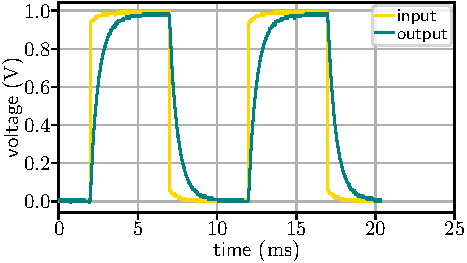
\includegraphics[width=\textwidth]{discharge.pdf}%
         \caption{capacitor charging and discharging measurement}\label{fig:decayd}%
     \end{subfigure}\hfill%
	  \begin{subfigure}[t]{0.495\textwidth}
         \centering
	     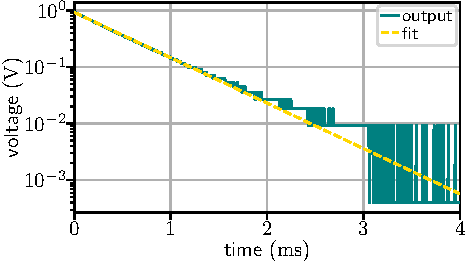
\includegraphics[width=\textwidth]{discharge_fit.pdf}
		  \caption{fit of the first discharge in figure \ref{fig:decayd} (time shifted)}\label{fig:decayfit}%
     \end{subfigure}%
	  \caption{capacitor charging and discharging}\label{fig:decay}%
\end{figure}
\subsection{Transfer Function}
Let $f_0 := 2\pi /\tau$.
For $f \in (0, \infty)$ and $U_\mathrm{in} =\SI{2}{\volt}$ we apply
\begin{equation*}
	U_\mathrm{in} \sin ( 2\pi f \bullet)
\end{equation*}
as input.
We wait for \SI{2}{\second} so that the transient settles and then measure the output.
From the theory section: The output has the (asymptotic) form
\begin{equation*}
	U_\mathrm{out} \sin (2 \pi f \bullet + \varphi),
\end{equation*}
where 
\begin{equation*}
	U_\mathrm{out} = \frac{1}{\sqrt{1+ f/f_0}} U_\mathrm{in}, \quad \varphi = - \arctan ( f /f_0).
\end{equation*}
To obtain $U_\mathrm{out}$ and $\varphi$ we do a least squares fit of the output signal.
We then repeat this procedure for different frequencies and fit the above relation (with $f_0$ as the parameter). The results can be found in figure \ref{fig:tf}.
  \begin{figure}
     \centering
     \begin{subfigure}{0.495\textwidth}
         %\centering
	     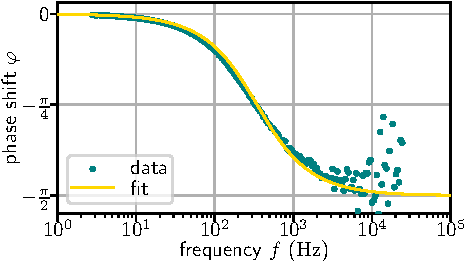
\includegraphics[width=\textwidth]{shifts.pdf}
         \caption{Phase shift fit}
     \end{subfigure}
	  \begin{subfigure}{0.495\textwidth}
         %\centering
	     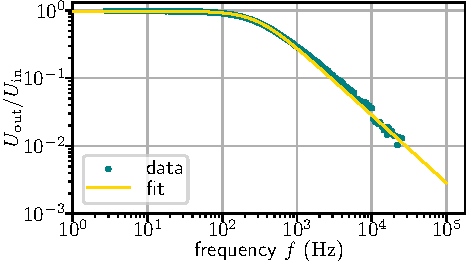
\includegraphics[width=\textwidth]{quots.pdf}
         \caption{Amplitude quotient fit}
     \end{subfigure}
	  \caption{Transfer function fit}
        \label{fig:tf}
\end{figure}
For the phase shift fit the optimal $\tau$ was $\tau = \SI{4.6 \pm 0.2 e-4}{\second}$.
For the amplitude quotient fit the optimal $\tau$ was $\tau = \SI{5.39 \pm 0.03 e-4}{\second}$.
\section{Inhomogeneous Solutions}
Let $G$ be the transfer function (from above) and $a \in (0, \infty)$.
Consider $u :[0, \infty) \to \mathbb{R}$, $u(t):=a t$ as input.
Let $y$ be the output of the system with initial value $0$ and input $u$.
Then (in some right half plane) $\hat y = G  \hat u$, where $\hat{}$ denotes Laplace transform.
Now $\hat u(s) = a s^{-2}$ for all $s \in \mathbb{C}_{\Re >0}$ and so for all $s \in \mathbb{C}_{\Re >0}$:
\begin{equation*}
	\hat y (s) = a s^{-2} \frac{1}{1+ \tau s}.
\end{equation*}
According to Wolfram-alpha (inverse Laplace) this implies for all $t\in[0, \infty)$:
\begin{equation*}
	y (t) = a(\tau ( e^{-t /\tau } -1) + t).
\end{equation*}
Measured by applying periodic signal with ramp first and then nothing (so the capacitor can fully discharge):
The results can be found in figure \ref{fig:rc_inhom}.
  \begin{figure}
     \centering
     \begin{subfigure}{0.495\textwidth}
         %\centering
	     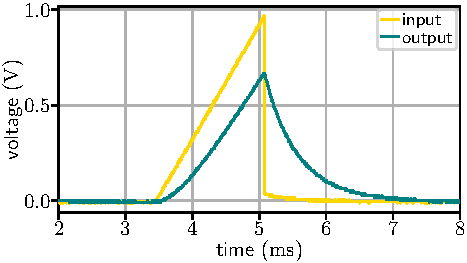
\includegraphics[width=\textwidth]{rc_inhom_ana.pdf}
	     \caption{measured data (periodic ramp)}
     \end{subfigure}
	  \begin{subfigure}{0.495\textwidth}
         %\centering
	     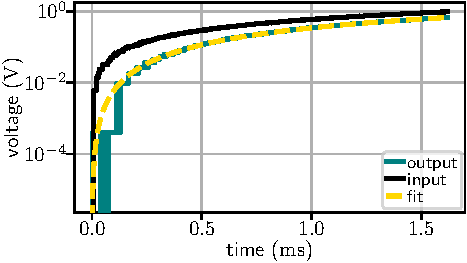
\includegraphics[width=\textwidth]{rc_inhom_fit.pdf}
		  \caption{fit of ramp on the left (time shifted)}
     \end{subfigure}
	  \caption{Inhomogeneous RC circuit}
        \label{fig:rc_inhom}
\end{figure}
\section{Linear Quadratic Optimal Control}
The CARE is:
\begin{equation*}
	\Pi^2 \mathcal{B}^2 - 2 \Pi^2 \mathcal{A}^2 - \mathcal{C}^2.
\end{equation*}
In this case the only non-negative solutions are:
\begin{equation*}
	\Pi = R \sqrt{\frac{1}{1-C^2}}.
\end{equation*}
Therefore the optimal control $u:[0, \infty) \to \mathbb{R}$ satisfies for all $t\in [0,\infty)$:
\begin{equation*}
	u (t) = - B \Pi \exp ( t (\mathcal{A}- \mathcal{B}^2 \Pi)).
\end{equation*}
\end{document}
